The main characteristic of LM rules is that they are constrained by the first
argument\footnote{In the implementation, the first argument of each fact is not
   stored.}. As shown in Fig.~\ref{fig:implementation:vm_overview}, each node
has its own database of linear facts (\emph{Linear DB}) and a database of
persistent facts (\emph{Persistent DB}).  Moreover, since only one thread at a
time will be using a node's database, we do not need to deal with
synchronization issues.

The databases of facts must be implemented efficiently because during matching
of rules we need to restrict the facts using \emph{join constraints}, which fix
arguments of predicates to instantiated values. Each node's database is
implemented using three kinds of data structures:

\begin{itemize}

\item \emph{Trie Data Structures} are used to store persistent facts. Tries are
   trees where facts are indexed by common prefix arguments.

\item \emph{Array Data Structures} are used to store persistent facts that are
   only derived as initial facts and used in rules LHS.

\item \emph{Doubly Linked List Data Structures} are used to store linear facts.
   We use a double linked list because it is a very efficient way to add and
   remove facts.

\item \emph{Hash Table Data Structures} are used to improve lookup when linked
   lists are too long and when we need to do search filtered by a fixed
   argument. The virtual machine decides which arguments are best to be indexed
   (see Section~\ref{sec:implementation:indexing}) and then uses a hash table
   indexed by the appropriate argument. If we need to go through all the facts,
   we just iterate through all the facts in the table. For collisions, we use
   the doubly linked list data structure mentioned above.

\end{itemize}

Figure~\ref{fig:implementation:hash_table} shows an example for a hash table
data structure for a \texttt{a(int,int)} predicate with 3 linear facts indexed
by the second argument and stored as a doubly linked list in bucket \texttt{2}.
Each linear fact contains the regular list pointers and the fact arguments.
Those are all stored continuously to improve data locality.

\begin{figure}[ht]
\centering
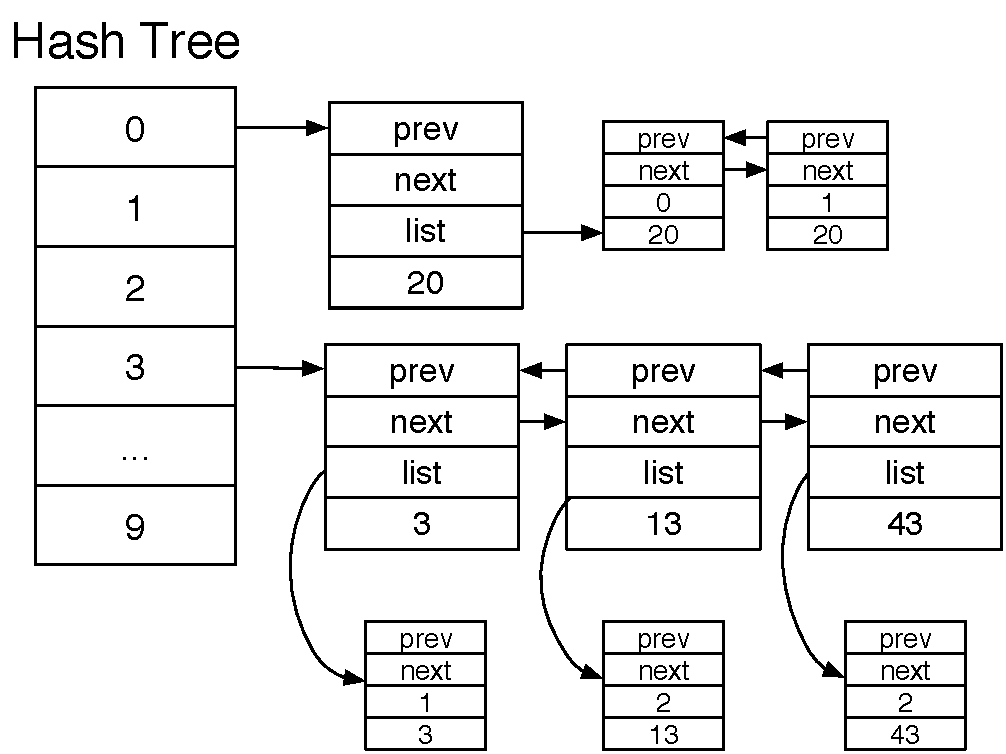
\includegraphics[width=0.6\textwidth]{figures/implementation/hash_table.pdf}
\caption{Hash table and doubly linked data structures for 
   a \texttt{a(int,int)} predicate.}
\label{fig:implementation:hash_table}
\end{figure}

\subsubsection{Locking}

Each node is protected by a main spin-lock that allows threads to change node
attributes. There is also a database spin-lock that protects the internal
database of the node and is locked whenever the node is in the \textbf{working}
state.  

To avoid unnecessary copying, when a node sends facts to a node located in
another thread, the current thread first attempts to lock the database lock of
the target node in order to directly update its database and indexing
structures, otherwise it adds the facts to the list of incoming facts that are
later processed by the owner thread of the target node.


%%%%%%%%%%%%%%%%%%%%%%%%%%%%%%%%%%%%%%%%%%%%%%%%%%%%%%%%%%%%%%%%%%%%%%

\subsection{Rule Engine}
\label{sec:implementation:rule_engine}

The rule engine decides which rules may need to be executed while taking into
account rule priorities. To understand how our engine works, consider the
following set of facts and rules:

\begin{Verbatim}[numbers=left,fontsize=\codesize]
a, e(1) -o b.  // rule 1
a -o c.        // rule 2
b -o d.        // rule 3
e(0) -o f.     // rule 4
c -o e(1).     // rule 5

a.
e(0).
\end{Verbatim}

Figure~\ref{fig:implementation:rule_engine} shows the rule engine data
structures for this example. The purpose of each data structure is as follows:

\begin{itemize}

   \item \texttt{Rule Queue} is the bitmap representing the rules scheduled to
      run. The $i^{th}$ is set if the $i^{th}$ rule is scheduled to run;

   \item \texttt{Rule Counter}, which keeps a count of the number of predicates
      needed by the rule that exist in the database. For the rule
      \texttt{a, e(1) -o b} then the rule needs predicates \texttt{a} and
      \texttt{e} and the rule counter is at the most 2 (where the rule can be
      executed).

   \item \texttt{Predicate Bitmap} is a bitmap representing the existence of a
      given predicate in the database;

\end{itemize}

\begin{figure}[t]
   \centering
   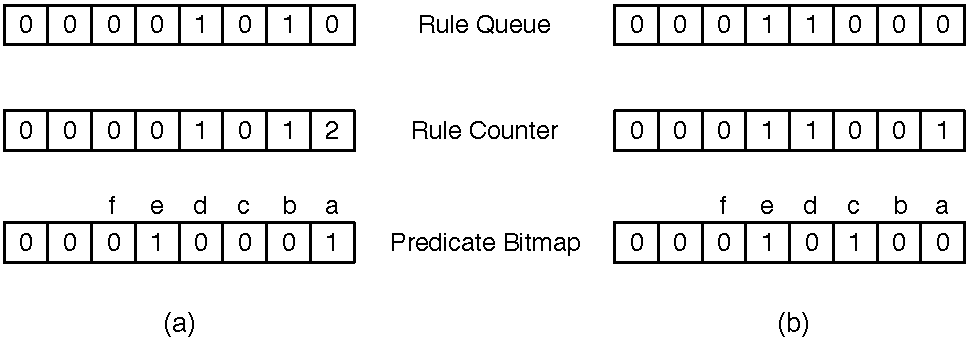
\includegraphics[width=0.8\textwidth]{figures/implementation/rule_queue.pdf}
   \caption{Rule engine data structures (a) before and (b) after applying 
      the rule \texttt{a -o c}.}
   \label{fig:implementation:rule_engine}
\end{figure}

Since we have facts for predicates \texttt{a} and \texttt{e}, the \texttt{Rules
Counter} starts with rules 1, 2 and 4 with 2, 1, 1 predicate counts. Since these
rules have the required counter to be applied, the \texttt{Rule Queue} bitmap
starts with the same three rules.  In order to pick rules for execution, we take
the rule corresponding to the least significant bit from the \texttt{Rule Queue}
bitmap, initially the first rule \texttt{a, e(1) -o b}. However, since we don't
have fact \texttt{e(1)}, this rule fails and its bit in \texttt{Rule Queue} must
be set to 0.  Figure~\ref{fig:implementation:rule_engine}(a) shows the rule
engine data structures at that point.

The next rule in \texttt{Rule Queue} is the second rule \texttt{a -o c}.
Because the this rule will succeed, we must consume fact \texttt{a} and derive
fact \texttt{c}. We thus update \texttt{Predicates Bitmap} accordingly, decrease
the counters for the first and second rule in \texttt{Rule Counter} since such
rules are no longer applicable (\texttt{a} was consumed), and increase the
counter for the fifth rule since \texttt{c} was derived. Finally, to update the
\texttt{Rule Queue}, we must schedule the fifth rule since its counter has been
increased to the required number (we have all predicates).  In the continuation,
the rule engine will schedule the fourth and fifth rules to run.
Figure~\ref{fig:implementation:rule_engine}(b) shows the rule engine data
structures at that point.

Note that every node in the program has the same set of data structures
presented in Fig.~\ref{fig:implementation:rule_engine}. We use 64 bit integers
to implement the 2 bitmaps and an array of 16 bits integers for \texttt{Rule
Counter}.

We do a small optimization to reduce the number of derivations of persistent
facts and, for that, we divide the program rules into two sets: \emph{persistent
rules} and \emph{non persistent rules}. Persistent rules are rules where only
persistent facts are involved. We compile such rules incrementally, i.e., we
attempt to fire all rules where a persistent fact is used. This is called the
\emph{pipelined semi-naive} evaluation and it originated in the P2
system~\cite{Loo-condie-garofalakis-p2}. This evaluation method avoids excessing
re-derivations of the same fact. The order of derivation does not matter for
those rules, since only persistent facts are used.

\subsection{Indexing}\label{sec:implementation:indexing}

To improve fact lookup, the VM employs a fully dynamic mechanism to
decide which argument may be optimal to index.  The algorithm is
performed in the beginning of execution and empirically tries to
assess the argument of each predicate that more equally spreads the
database across the values of the argument.  A single thread performs
the algorithm for all predicates.

The indexing algorithm is performed in three main steps. First, it
gathers lookup statistics by keeping a counter for each
predicate's argument.  Every time a fact search is performed where
arguments are fixed to a value, the counter of such arguments is
incremented. This phase is performed during rule execution for a small
fraction of the nodes in the program.

The second step of the algorithm selects the candidate arguments of each
predicate.  If a predicate was not searched with any fixed arguments, then it
will be not indexed and there are no candidates.  If only one argument was
fixed, then such argument is the only available candidate argument and thus
immediatelly becomes the indexing argument. Otherwise, the top 2 arguments are
selected for the third phase, where \emph{entropy statistics} are collected
dynamically.

During the third phase, each candidate argument has an entropy score.
Before a node is executed, the facts of the target predicate
are used in the following formula applied for the two arguments:

\[
Entropy(A, F) = - \sum_{v \in values(F, A)} \frac{count(F, A = v)}{total(F)} \log_2 \frac{count(F, A = v)}{total(F)}
\]

\noindent where $A$ is the target argument, $F$ is the set of linear facts for
the target predicate, $values(F, A)$ is set of values of the argument $A$,
$count(F, A = v)$ counts the number of linear facts where argument $A$ is equal
to $v$ and $total(F)$ counts the number of linear facts in $F$.  The entropy
value is a good metric because it tells us how much information is needed to
describe an argument. If more information is needed, then that must be the best
argument to index.

For one of the arguments to score, $Entropy(A, F)$ multiplied by the number of
times it has been used for lookup, must be larger than the other argument. The
argument with the best score is selected and then a global variable called
\texttt{indexing\_epoch} is updated. In order to convert the node's linked lists
into hash tables, each node also has a local variable called
\texttt{indexing\_epoch} that is compared to the global variable in order to
rebuild the database according to the new indexing information.

The VM also dynamically resizes the hash table if necessary. When the hash table
becomes too dense, it is doubled in size. When it becomes too sparse, it is
reduced in half or simply transformed back into a doubly linked list. This is
done once in a while, before a node executes.

We have seen very good results with this scheme. The overhead of dynamic
indexing is negligible since programs run almost as fast as if the indices have
been added from the start. However, the programmer can still index predicates
statically, if needed.
